\documentclass{article}

% if you need to pass options to natbib, use, e.g.:
%     \PassOptionsToPackage{numbers, compress}{natbib}
% before loading neurips_2020

% ready for submission
% \usepackage{neurips_2020}

% to compile a preprint version, e.g., for submission to arXiv, add add the
% [preprint] option:
%     \usepackage[preprint]{neurips_2020}

% to compile a camera-ready version, add the [final] option, e.g.:
%     \usepackage[final]{neurips_2020}

% to avoid loading the natbib package, add option nonatbib:
\usepackage[final, nonatbib]{neurips_2020}

\usepackage[utf8]{inputenc} % allow utf-8 input
\usepackage[T1]{fontenc}    % use 8-bit T1 fonts
\usepackage{hyperref}       % hyperlinks
\usepackage{url}            % simple URL typesetting
\usepackage{booktabs}       % professional-quality tables
\usepackage{amsfonts}       % blackboard math symbols
\usepackage{nicefrac}       % compact symbols for 1/2, etc.
\usepackage{microtype}      % microtypography
\usepackage{graphicx}
\usepackage{float}
\usepackage{biblatex}
\usepackage[utf8]{inputenc}
\usepackage[english]{babel}


\addbibresource{refs.bib}

\title{Graph-based Neural Networks for Retrosynthesis Planning: A Comprehensive Review and Comparative Analysis}

% The \author macro works with any number of authors. There are two commands
% used to separate the names and addresses of multiple authors: \And and \AND.
%
% Using \And between authors leaves it to LaTeX to determine where to break the
% lines. Using \AND forces a line break at that point. So, if LaTeX puts 3 of 4
% authors names on the first line, and the last on the second line, try using
% \AND instead of \And before the third author name.

\author{
  Xun Zhou\\
  Department of Computer Science\\
  Shanghai Jiao Tong University\\
  X21 \\
  \texttt{chosen@sjtu.edu.cn} \\
  % examples of more authors
  % \And
  % Coauthollr \\
  % Affiliation \\
  % Address \\
  % \texttt{email} \\
  % \AND
  % Coauthor \\
  % Affiliation \\
  % Address \\
  % \texttt{email} \\
  % \And
  % Coauthor \\
  % Affiliation \\
  % Address \\
  % \texttt{email} \\
  % \And
  % Coauthor \\
  % Affiliation \\
  % Address \\
  % \texttt{email} \\
}

\begin{document}
\maketitle
\linespread{1.5}
\begin{abstract}
  In this project, we implemented LocalRetro method for single-step retrosynthesis prediction, and an MLP based neural network for Molecule evaluation. LocalRetro demonstrates promising results, but MLP performs poorly in our experiments.

\end{abstract}
  

\section{Introduction}

The pursuit of designing molecules and materials with desired properties is a crucial goal in chemistry and materials science. Cheminformatics leverages data to uncover the intricate relationship between molecular structures and their properties, enabling the discovery of novel functional molecules. Machine learning has revolutionized this field by rapidly predicting molecular properties based on their structures and even reverse-engineering molecules from desired functionalities. However, synthesis planning remains a crucial step to bridge the gap between theoretical designs and practical implementation. The retrosynthesis problem inherently poses challenges as it involves a one-to-many mapping, which means that there can be multiple possible reaction pathways to synthesize a target compound. This aspect adds complexity and makes the task more difficult.

% A chemical reaction can be understood as a map that transforms a set of $N$ reactant molecules, denoted as $\{R_i\}_{i=1}$, into a single outcome molecule, denoted as $O$. In this paper, we specifically focus on reactions with a single outcome, as it is a common formulation in retrosynthetic analysis. The reaction centers refer to the specific atoms or bonds that undergo changes during the reaction. Given a reaction, we can define the template of it as:

% $$T:= o^T \rightarrow r_1^T + r_2^T + \ldots + r_{N(T)}^T$$

% where $N(\cdot)$ denotes the count of reactant subgraphs present in the template. 
% Typically, we can consider the subgraph pattern $o^T$ as the isolated reaction center derived from $O$, while $r_i\in T$, where $i \in {1, 2, ..., N(T)}$, represents the associated pattern within the i-th reactant. However, it is worth noting that in practice, these patterns may also encompass neighboring structures of the reaction centers.

\section{Related Works}

GNNs have emerged as a powerful tool for solving this problem by leveraging the graph structure of molecules. In a graph representation of a molecule, atoms are represented as nodes, and bonds between atoms are represented as edges connecting the nodes. GNNs can effectively capture the structural information and relationships between atoms in a molecule graph.

One popular GNN model used in Retrosynthetic Reaction Prediction is the Graph Convolutional Network (GCN). The GCN applies convolutional operations on the graph to propagate and update information across nodes. The key idea behind GCN is to aggregate and combine information from neighboring nodes to compute new node representations. The propagation rule can be formulated as follows:

\begin{equation}
  h_i^{(l+1)} = \sigma\left(\sum_{j\in \mathcal{N}(i)}\frac{1}{c_{ij}}W^{(l)}h_j^{(l)}\right)
\end{equation}

In the above formula, $h_i^{(l+1)}$ represents the updated representation of node i at layer $l+1, h_j^{(l)}$ represents the representation of neighboring node $j $ at layer $l, \mathcal{N}(i)$ represents the neighbors of node $i, W^{(l)}$ represents the weight matrix at layer $l, c_{ij}$ is a normalization constant, and $\sigma$ is a non-linear activation function.

To predict retrosynthetic reactions, GNN models are trained on a large dataset of known reactions. The model learns to encode the structure of the reactant molecules and predict the product molecules. During inference, the GNN model takes a target molecule as input and predicts a set of precursor molecules along with the corresponding reaction steps.

By effectively capturing the graph structure of molecules and learning from a large number of known reactions, GNN-based models have shown promising results in Retrosynthetic Reaction Prediction. They have the potential to accelerate the process of drug discovery and synthesis planning by providing guidance on feasible reaction pathways for target molecules.

Please note that the formula provided above represents a simplified version of the propagation rule used in GCN. Different variations of GNNs may have slightly different formulations, but the underlying idea of aggregating information from neighboring nodes remains consistent.

% \subsection{Conditional Graph Logic Network}

% Conditional Graph Logic Network is a graph neural network based method in which the probability of the predicted template and precursor is determined based on the probability of the reaction template given a molecule and the probability of the reactant given a molecule and template. That is:
% \begin{equation}
%   p(T | O) \propto \exp(w_1(T, O)) \cdot \phi_O(T) 
% \end{equation}
% \begin{equation}
% p(R | T, O) \propto \exp(w_2(R, T, O)) \cdot \phi_{O,T}(R)
% \end{equation}
% \begin{equation}
%  p(R, T | O) \propto \exp(w_1(T, O) + w_2(R, T, O)) \cdot \phi_O(T) \cdot \phi_{O,T}(R)
% \end{equation}
% The number of templates and reactants that can be predicted may vary depending on the specific molecule conditions.

% We can further decompose and separate parameters, the expression can be written as:

\section{Methods}

\subsection{Task 1: LocalRetro}

We employ the LocalRetro algorithm to solve the single-step retrosynthesis prediction problem. We leverage the fact that reactant molecules retain a significant portion of their substructures and fragments during and after a reaction. This allows us to concentrate on the changes in the molecular structure, specifically the alterations in atoms or bonds, to facilitate retrosynthesis. Rather than starting from scratch to identify suitable reactants, our focus is on deducing the specific local changes that took place to generate the given product. These changes can involve the formation or breaking of bonds and/or the addition or removal of atoms. By analyzing and understanding these structural transformations, we can effectively navigate the retrosynthetic process.

We leverage the domain-specific knowledge extracted by the original authors, such as reaction templates, to classify reactions. This approach significantly improves the classification performance by reducing the complexity of the task. Instead of dealing with thousands of distinct templates, we can now categorize reactions into 657 classes, thanks to the utilization of these extracted templates.

Next, the new model concentrate more on local environments,  predict the correct local reaction template at each atom and bond that leads to the given product. We represent the molecule as a heterogeneous graph $G = (V,E)$ with $V$(vertices) denoting atoms and $E $(edges) denoting bonds. To encode the surrounding environmental information for each atom,a message passing neural network (MPNN) is used to described to update each atom feature. We denote the message passing function by $MPNN(\cdot)$, with the atomic features of atom $a$ as $v_a$, the atomic features of its neighboring atom $b$ as $v_b$, and the features of their connecting bond as $e_{ab}$. The atomic features of atom $a$ are updated by the MPNN via:
\begin{equation}
  v_a' = MPNN(v_a, \{v_b\}, \{e_{ab}\})
\end{equation}
$\{ \}$ denotes a set of neighboring atoms around a given atom. After the atomic features are updated, the bond feature is represented by concatenating two atomic features  $(v_a' || v_b')$ and goes through a fully connected layer.
\begin{equation}
e_{ab}' = w(v_a' || v_b') + c
\end{equation}
Where  $w$ is the weights and $ c$  is the bias of the fully connected layer.

To incorporate the global dependency and nonlocality of reactions, the model employ a global attention mechanism to update the atomic features, denoted as $x_a$, and bond features, denoted as $x_{ab}$. The update process can be expressed as:
\begin{equation}
x_a' = GRA(x_a, \{v_a'\}, \{e_{ab}'\})
\end{equation}
\begin{equation}
x_{ab}' = GRA(e_{ab}', \{v_a'\}_{a \in V}, \{e_{ab}'\}_{ab \in E})
\end{equation}
where GRA($\cdot$) represents the application of the global attention mechanism using the current atomic features $x_a$, the set of all updated atomic features is $\{v_a'\}$, and the set of all updated bond features is $\{e_{ab}'\}$.

Next comes the typical step of training classifiers using the extracted features.Separate classifiers for atom reaction templates and bond reaction templates are used to compute their respective outputs. These classifiers utilize the updated representations of atoms and bonds.Given the nature of the problem, we used cross-entropy loss to measure the performance of the model.

\subsection{Task 2: MLP}

We utilize a multilayer perceptron (MLP) to learn molecule evaluation in a supervised manner. Due to the significant difference in the value distribution between the training and test domains, I attempted to apply z-score normalization to both the values in their respective domains. Subsequently, I fed the normalized data into an MLP for supervised learning.

We used the unpacked Morgan FingerPrint as the input and apply layer normalization at each layer of the MLP. The ReLU activation function is used. We also utilize the Mean Squared Error (MSE) loss function.

\begin{table}[H]
  \centering
  \caption{The training and test datasets exhibit different data distributions.}
  \begin{tabular}{ccccc}
  \hline
  \multicolumn{1}{|c|}{Model}     & \multicolumn{1}{c|}{min} & \multicolumn{1}{c|}{max}   & \multicolumn{1}{c|}{mean} & \multicolumn{1}{c|}{std}  \\ \hline
  \multicolumn{1}{|c|}{Train set} & \multicolumn{1}{c|}{0}   & \multicolumn{1}{c|}{44.67} & \multicolumn{1}{c|}{0.46} & \multicolumn{1}{c|}{1.27} \\ \hline
  \multicolumn{1}{|c|}{Test set}  & \multicolumn{1}{c|}{0}   & \multicolumn{1}{c|}{45.2}  & \multicolumn{1}{c|}{1.93} & \multicolumn{1}{c|}{3.1}  \\ \hline
  \multicolumn{1}{l}{}            & \multicolumn{1}{l}{}     & \multicolumn{1}{l}{}       & \multicolumn{1}{l}{}      & \multicolumn{1}{l}{}     
  \end{tabular}
  \end{table}


\section{Expriment and Discuss}

\subsection{Task 1}

Given the limited time available, We trained the model for only 3 epochs. Despite the incomplete convergence, the model has shown impressive performance.

\begin{table}[H]
  \caption{predict accuracy in task 1}
  \centering
  \begin{tabular}{cccccl}
  \hline
  \multicolumn{1}{|c|}{k}        & \multicolumn{1}{c|}{1}     & \multicolumn{1}{c|}{3}     & \multicolumn{1}{c|}{5}     & \multicolumn{1}{c|}{10}     & \multicolumn{1}{l|}{50}    \\ \hline
  \multicolumn{1}{|c|}{accuracy} & \multicolumn{1}{c|}{0.345} & \multicolumn{1}{c|}{0.516} & \multicolumn{1}{c|}{0.566} & \multicolumn{1}{c|}{0.6090} & \multicolumn{1}{l|}{0.627} \\ \hline
  \multicolumn{1}{l}{}           & \multicolumn{1}{l}{}       & \multicolumn{1}{l}{}       & \multicolumn{1}{l}{}       & \multicolumn{1}{l}{}        &                           
  \end{tabular}
  \end{table}


In this model, we incorporate more prior knowledge by emphasizing the correlation between chemical properties and neighboring atoms. We preserve more connections between neighboring atoms and chemical bonds to capture local dependencies. Additionally, we leverage attention mechanisms to prevent important long-range correlations from being overlooked. We believe that this is one of the key factors contributing to the success of this model compared to other graph-based models. By effectively incorporating prior knowledge and leveraging attention, we can capture both local and global information, leading to improved performance in handling chemical structures and properties.

\subsection{Task 2}


\begin{figure}[H]
  \centering
  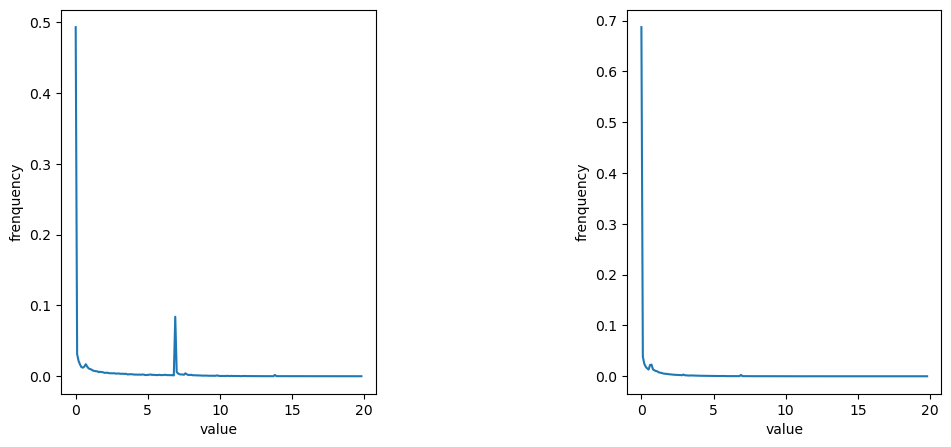
\includegraphics[width=0.8\textwidth]{f.png}
  \caption{The training(right) and testing(left) datasets exhibit different data distributions.}
\end{figure}
\subsection{Training and evaluation}

The performance of the model used in Task 2 is unsatisfactory, as there is minimal improvement in the loss on the test set. We believe there could be two possible reasons for this.

Firstly, there is a significant disparity in the data distribution between the training and test sets. The training set is more concentrated around zero, while the test set exhibits higher variance, with many data points distributed around seven. To improve the performance, it may be necessary to explore more transfer learning techniques or expand the dataset to better capture the variability in the test set.

Secondly, the Morgan FingerPrint used as input may be too sparse for effective processing by the multilayer perceptron (MLP). MLPs may not be well-suited for handling such sparse data. Considering alternative methods like graph neural networks (GNNs) may yield better results, as GNNs are specifically designed to process graph-structured data and can better capture the structural information inherent in the Morgan FingerPrint.


\section{Contribution}

Xun Zhou 517082910012 100\%

code: https://github.com/chosen66/Retrosynthetic-Planning


\end{document}
